\section{Theorie}
\label{sec:Theorie}

\subsection{Grundprinzip}
Ein Laser (\textit{light amplification by stimulated emisson of radiation}) besteht hauptsächlich aus drei Komponenten.
Das \textit{aktive Medium}, welches von einer \textit{Energiepumpe} mit Energie gespeißt wird, sorgt für eine Besetzungsinversion zwischen mindestens zwei Energienivieaus im Medium. Der \textit{Resonator} sorgt schließlich über Hin- und Herreflektion dafür, dass das Licht möglichst häufig durch das aktive Medium hindurchgeht. Über einen Spiegel mit geringer Durchlässigkeit kann das Licht den Aufbau \ref{fig:auf} verlassen.

\begin{figure}
    \centering
    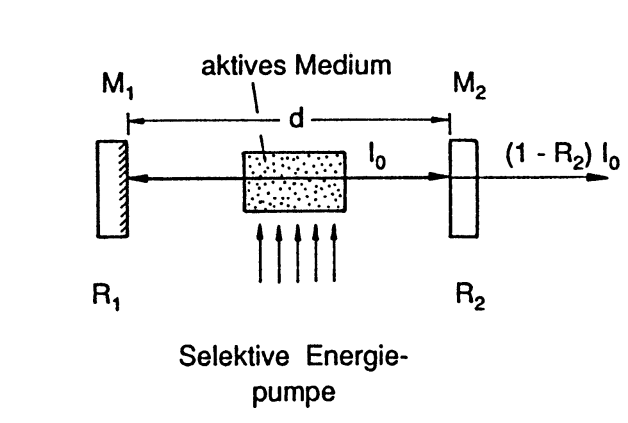
\includegraphics[width=8cm]{Bilder/Aufbau.PNG}
    \caption{Schematischer Aufbau des Lasers.\cite{Laserspektroskopie_1}}
    \label{fig:auf}
\end{figure}

\subsection{Das Aktive Medium}
Für die Funktionsweise eines Lasers sind drei Prozesse der Wechselwirkung zwischen Licht und Materie besonders wichtig:
\begin{itemize}
    \item Absorbtion:

    Trifft Licht auf ein Atom im Grundzustand, dessen Energie der Energiedifferenz zwischen Grundzustand und nächstem Energienivieau entspricht, wird dieses Licht aborbiert und das jeweilge Elektron wird auf das jeweilige Energienivieau gehoben. Dadurch geht das Atom in einen angeregten Zustand über.

    \item spontane Emission:

    Angeregte Atome fallen ohne äußeren Einfluss in ihren Grundzustande zurück und emittieren dabei ein Photon, dessen Energie wieder der Energiedifferenz zwischen den beiden Niveaus entspricht. Die spontane Emission geschieht zufällig und ist nur an eine Emissionswahrscheinlichkeit geknüpft. 

    \item induzierte Emission:

    Trifft ein Photon auf ein angeregtes Atom, dessen Energie der Energiedifferenz zwischen zwei Zuständen entspricht, so geht das Atom in den jeweils geringeren Zustand über und emittiert dabei ein Photon gleicher Richtung, Polarisation und Wellenlänge.(Abbildung \ref{fig:ver})
\end{itemize}

\begin{figure}
    \centering
    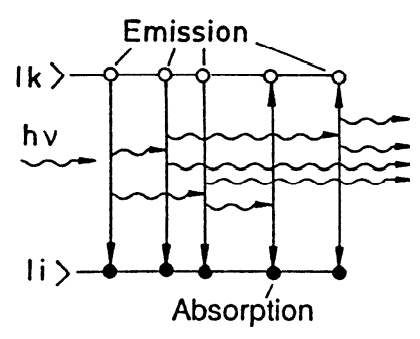
\includegraphics[width=6cm]{Bilder/verstaerkung.PNG}
    \caption{Prinzip der Verstärkung durch induzierte Emission.\cite{Laserspektroskopie_1}}
    \label{fig:ver}
\end{figure}

Damit es zu einer Verstärkung kommen kann, muss eine Besetzungsinversion im aktiven Medium erzeugt werden . Ohne äußeren Einfluss sind die Zustände der Atome im Medium gemäß der Boltzmann-Verteilung verteilt. Atome in Zuständen geringerer Energie kommen also häufiger vor, als welche in Zuständen höherer Energie. in dem Fall wäre die Erzeugung von induzierten Emissionen unwahrscheinlich und es käme zu keiner Verstärkung.
Die Energiepumpe sorgt dafür, dass ein Niveau höherer Energie häufiger besetzt vorkommt, als ein Niveau niedrigerer Energie (Abbildung \ref{fig:inv}). Dadurch steigt die Wahrscheinlichkeit für jedes Photon im Medium, auf ein angeregtes Atom zu treffen und dadurch eine Emission zu induzieren. Je nach Wahl des aktiven Mediums ist auch die Energiedifferenz zwischen diesen beiden Niveaus eine andere. Dadurch ist das Medium entscheident für die Wellenlänge des vom Laser ausgestrahlten Lichtes.

\begin{figure}
    \centering
    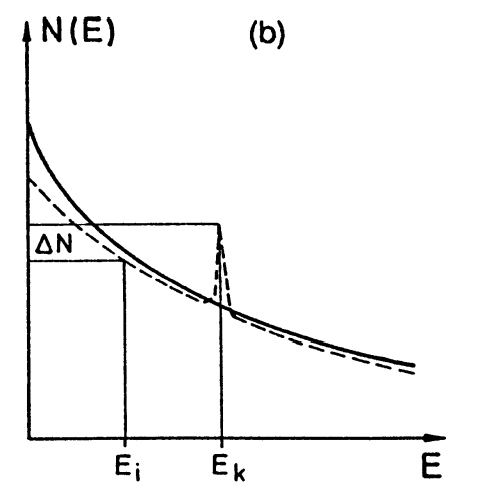
\includegraphics[width=6cm]{Bilder/Inversion.PNG}
    \caption{Verteilung der Zustände gemäß Boltzmann-Verteilung und gemäß Besetzungsinversion.\cite{Laserspektroskopie_1}}
    \label{fig:inv}
\end{figure}

\subsection{Stabilität des Resonators}
Der Resonator besteht aus zwei Spiegeln, welche unterschiedliche Krümmungen besitzen können. Damit das Licht stabil im Resonator oszillieren kann, dürfen die Spiegel nur innerhalb gewisser Abstände zueinander sein. Sonst würde der zu große Verlust zu einem erliegen der Laser-Tätigkeit führen. in diesem Fall (kleine Spiegel gegenüber dem Abstand) wird der hauptsächliche Verlust durch Beugung verursacht.
Für die Stabilität des Resonators muss die Ungleichung
\begin{equation}
    \label{eqn:g}
   0 \leq g_1 \cdot g_2 \leq 1
\end{equation}
erfüllt sein. Dabei ist $g$ der Stabilitätsparameter, der sich aus dem Abstand beider Spiegel $L$ und dem jeweilgen Krümmungsradius $b$ zusammensetzt:
\begin{equation}
    g_i = 1-\frac{L}{b_i}.
\end{equation}

Für die Krümmungsradien

\begin{align*}
    b_1 & = \infty \\
    b_2 & = \SI{100}{\centi\m} \\
    b_3 & = \SI{140}{\centi\m}
\end{align*}

sind für verschiedene Spiegelkonstellationen die Stabilitätsbedingung \eqref{eqn:g} in Abbildung \ref{fig:vor} in Abhängigkeit des Spiegelabstandes aufgetragen.

\begin{figure}
    \centering
    \includegraphics[width=\textwidth]{build/Vorbereitung_Stabilität.pdf}
    \caption{Stabilitätsparameter von verschiedenen Spiegelkonstallation in Abhängigkeit des Spiegelabstandes.}
    \label{fig:vor}
\end{figure}

Für die Spiegelkonstallation ($g_3$,$g_3$) folgt die Bedingung
\begin{equation}
    0 \leq L \leq \SI{280}{\cm}
\end{equation}
und für die Spiegelkonstallation ($g_1$,$g_3$) die Bedingung
\begin{equation}
    0 \leq L \leq \SI{140}{\cm}.
\end{equation}
Dabei ist zu Beachten, dass ($g_3$,$g_3$) die Stabilitätsgrenze bei $L = \SI{140}{\cm}$ berührt. Theoretisch ist der Resonator dort noch stabil, jedoch kann es in der Praxis auf Grund von kleinen Ungenauigkeiten trotzdem zu einem Stabilitätsverlust kommen.


\subject{Moden im Resonator}

Der Resonator begrenzt durch seinen Spiegelabstand auch die maximale Wellenlänge des im Resonator befindlichen Lichtes. Desshalb kann dieses Licht nur in diskreten Moden (TEM) auftauchen. 
Die Intensitätsverteilung im Zentrum und entlang einer Achse ($n=0$) des Resonators ist proportional zu dem Ausdruck 
\begin{equation}
    \label{eqn:mode}
    I_{0,m}(L) \propto I_0 H_m^2\left(\frac{\sqrt{2}L}{\omega}\right)\exp{\left(-\frac{L^2}{\omega^2}\right)},
\end{equation}
wobei $H_m$ das m-te Hermitepolynom und $\omega$ die Strahldivergenz darstellt. $L$ ist der Abstand vom Zentrum und $I_0$ die Maximalintensität.

\subsection{Helium-Neon-Laser}
Im Fall des He-Ne-Lasers wird als aktives Medium ein Gemisch aus gasförmigem Helium und Neon in einem Verhältnis von ca 5:1 verwendet.
Über elektrische Entladungen werden die Helium Atome in angeregte Zustände versetzt. Diese Atome stoßen wiederum mit den Neon-Atomen, welche ihrerseits in angeregte Zustände versetzt werden (Stoß 2. Art). Dadurch kommt es zu der notwendigen Besetzungsinversion. Die hauptsächlichen Zustandsübergänge sind in Abbildung \ref{fig:linie} dargestellt.

\begin{figure}
    \centering
    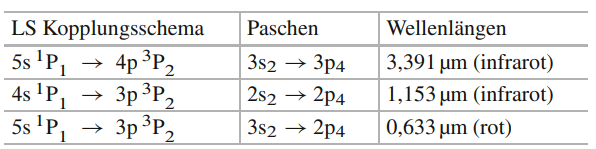
\includegraphics[width=\textwidth]{Bilder/linie.PNG}
    \caption{Übergänge der intensivsten Linien des Neons.\cite{Laser}}
    \label{fig:linie}
\end{figure}

Der gesamte Aufbau eins He-Ne-Laser ist in Abbildung \ref{fig:he} dargestellt.

\begin{figure}
    \centering
    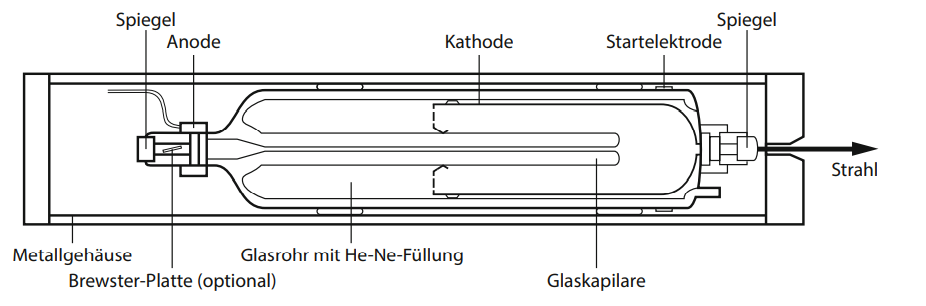
\includegraphics[width=\textwidth]{Bilder/he.PNG}
    \caption{Aufbau eines He-Ne-Lasers.\cite{Laser}}
    \label{fig:he}
\end{figure}


\subsection{Wellenlänge}

Wie bereits erwähnt wird die Wellenlänge des Lasers hauptsächlich durch die Wahl des aktiven Mediums bestimmt. 
Die Wellenlänge des Lichtes kann mit Hilfe eines Gitters bestimmt werden. Dabei lässt sich die Wellenlänge über die Relation
\begin{equation}
    \label{eqn:lamb}
    \lambda = \frac{g\sin{\left(\arctan{\left(\frac{d_k}{L}\right)}\right)}}{k}
\end{equation}
bestimmen. Dabei ist $g$ die Gitterkonstante, $d_k$ der Abstand vom Mittelpukt bis zum k-ten Maximum und $L$ der Abstand zwischen dem Gitter und dem Schirm.

\subsection{Polarisation}

Licht kann unterschiedlich polarisiert sein. Trifft linear polarisiertes Licht auf einen Polarisationsfilter, so wird in Abhängigkeit des Winkels $\phi$ zwischen Filter und Polarisationsrichtung nur ein Teil des Lichtes durch den Filter gelangen. Die Intensität der durchgelassenen Strahlung lässt sich über das \textit{Gesetz von Malus}
\begin{equation}
    \label{eqn:pol}
    I = I_0\cos^2{(\phi)}
\end{equation}
bestimmen.
%In knapper Form sind die physikalischen Grundlagen des Versuches, des Messverfahrens, sowie sämtliche für die Auswertung erforderlichen Gleichungen darzustellen. (Keine Herleitung)

%(eventuell die Aufgaben)

%Der Versuchsaufbau: Beschreibung des Versuchs und der Funktionsweise (mit Skizze/Bild/Foto)
